\documentclass{beamer}

\usepackage{amsmath}
\usepackage[english]{babel}
\usepackage{unicode-math}
\usepackage{mathtools}
\usepackage{derivative}

\usetheme{metropolis}

\setmainfont{Stix Two Text}
\setmathfont{Stix Two Math}

\DeclarePairedDelimiter{\ceil}{\lceil}{\rceil}
\DeclarePairedDelimiter{\floor}{\lfloor}{\rfloor}
\DeclarePairedDelimiter{\abs}{\lvert}{\rvert}
\DeclarePairedDelimiter{\norm}{\lVert}{\rVert}
\DeclarePairedDelimiter{\bra}{\langle}{\rvert}
\DeclarePairedDelimiter{\ket}{\lvert}{\rangle}
\DeclarePairedDelimiter{\expval}{\langle}{\rangle}
\DeclarePairedDelimiter{\norder}{\mathcolon}{\mathcolon}
\DeclarePairedDelimiter{\anorder}{\typecolon}{\typecolon}
	
\newcommand{\laplace}{\mbfnabla^2}
\newcommand{\trans}{{\scriptscriptstyle\mathsf{T}}}

\newcommand{\conv}{\ast}
\newcommand{\vdot}{\cdot}
\newcommand{\vcross}{\vectimes}
\newcommand{\vb}[1]{\symbfup{#1}}
\newcommand{\vu}[1]{\hat{\vb{#1}}}
\newcommand*\dd[2][\relax]{\mathop{\ifx\relax#1\odif{#2}\else \odif[order={#1}]{#2}\fi}}

\newcommand{\vacket}{\ket*{0}}
\newcommand{\vacbra}{\bra*{0}}

\DeclareMathOperator{\trace}{Tr}
\DeclareMathOperator{\sinc}{sinc}

\AtBeginDocument{
	\let\Re\relax
	\let\Im\relax
	\DeclareMathOperator{\Re}{Re}
	\DeclareMathOperator{\Im}{Im}

	\renewcommand{\div}{\mathop{\mbfnabla\vdot}}
	\newcommand{\curl}{\mathop{\mbfnabla\vectimes}}
}

\DeclarePairedDelimiterX{\comm}[2]{[}{]}{#1,#2}

\DeclarePairedDelimiterX{\braket}[2]{\langle}{\rangle}{#1\delimsize\vert#2}
\DeclarePairedDelimiterX{\ketbra}[1]{\lvert}{\rvert}{#1\rangle\delimsize\langle#1}


\usetikzlibrary{arrows.meta,fit,positioning}

\title{A theoretical framework for quantum-optical communication - towards CV-QKD}
\date{\today}
\author{Bodo Kaiser}
\institute{Ludwig-Maximilians-Universität München}

\begin{document}
	\maketitle
	
	\begin{frame}
		\begin{center}
			\textbf{Prelude}
			
			What is light?
		\end{center}
	\end{frame}
	
	\section{Introduction}
	
	\begin{frame}{Secure communication}
		\begin{figure}
		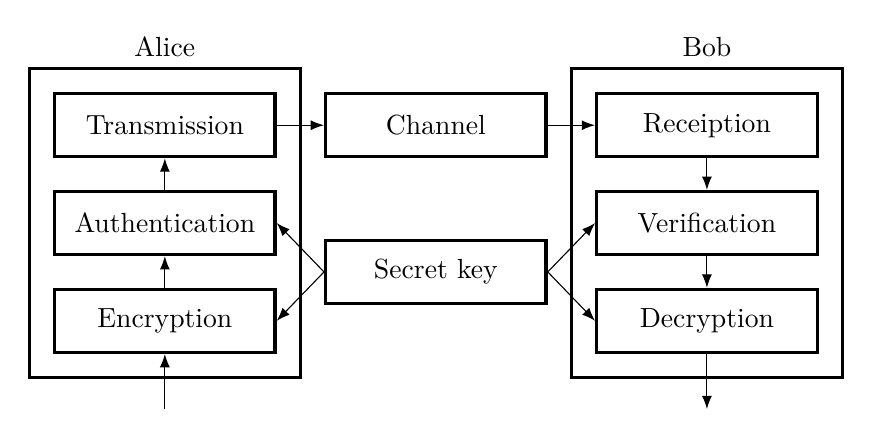
\begin{tikzpicture}[
			node distance=4mm,
			block/.style={draw, very thick, minimum width=28mm, minimum height=8mm},		
			superblock/.style={draw, very thick, inner sep=3mm},
		]
			\coordinate (in);
			\node[block, above=7mm of in] (encryption) {Encryption};
			\node[block, above=of encryption] (authentication) {Authentication};
			\node[block, above=of authentication] (transmitter) {Transmission};
			\node[block, right=6mm of transmitter] (channel) {Channel};
			\node[block, right=6mm of channel] (receiver) {Receiption};
			\node[block, below=of receiver] (verification) {Verification};
			\node[block, below=of verification] (decryption) {Decryption};
			\coordinate[below=7mm of decryption] (out);

			\path (encryption) -- (verification) node[midway, block] (key) {Secret key};

			\draw[-Latex] (key.west) -- (encryption.east);
			\draw[-Latex] (key.west) -- (authentication.east);
			\draw[-Latex] (key.east) -- (decryption.west);
			\draw[-Latex] (key.east) -- (verification.west);
			
			\draw[-Latex] (in) -- (encryption);
			\draw[-Latex] (encryption) -- (authentication);
			\draw[-Latex] (authentication) -- (transmitter);
			
			\draw[-Latex] (decryption) -- (out);
			\draw[-Latex] (verification) -- (decryption);
			\draw[-Latex] (receiver) -- (verification);
	
			\draw[-Latex] (transmitter) -- (channel.west);
			\draw[-Latex] (channel.east) -- (receiver);
			
			\node[superblock, label={Alice}, fit=(encryption) (transmitter)] {};
			\node[superblock, label={Bob}, fit=(decryption) (receiver)] {};
		\end{tikzpicture}
			\caption{Block diagram of a transmission system ensuring integrity and confidentiality of the transmitted using authentication and encryption, requiring a secret key.}
		\end{figure}
	\end{frame}
	
	\begin{frame}{Key distribution problem}
		% public-key distribution
	\end{frame}
	
	\begin{frame}{Quantum key distribution}
		Main idea of QKD:
		- boson or qubit state
		- quantum transmission
		- post-processing
	\end{frame}
	
	\begin{frame}{Polarization-encoding qubit-based QKD}
		
	\end{frame}
	
	\begin{frame}{Squeezing-encoding boson-based QKD}
		
	\end{frame}
	
	\begin{frame}{Coherent-encoding boson-based QKD}
		
	\end{frame}
	
	\begin{frame}{Problem statement}
		Venn-diagram of disciplines
		and 
		conflict
	\end{frame}
	
	\section{Classical communication theory}
	
	\section{Quantum theory of light}
	
	\section{Quantum theory of electro-optics}
	
	\section{Quantum communication theory}
	
	\section{Conclusion}
	
	\begin{frame}
		\begin{center}
			\textbf{Postlude}
			
			How does light interact with matter?
		\end{center}
	\end{frame}
\end{document}